\documentclass[11pt,a4paper]{article}
\usepackage[utf8]{inputenc}
\usepackage[T1]{fontenc}
\usepackage[french]{babel}
\usepackage{geometry}
\usepackage{graphicx}
\usepackage{booktabs}
\usepackage{amsmath}
\usepackage{amssymb}
\usepackage{hyperref}
\geometry{margin=2.4cm}

\title{Recodage de Bouchaud--Mézard\\\large Wealth condensation in a simple model of economy}
\author{Recodage Python: numpy, scipy, matplotlib}
\date{1 juillet 2026}

\begin{document}
\maketitle

\section{Objectif}

L'article étudie une dynamique stochastique de richesse
\[
  \frac{dW_i}{dt}=\eta_i(t)W_i+\sum_{j\ne i}J_{ij}W_j-\sum_{j\ne i}J_{ji}W_i,
\]
et montre que le modèle produit des queues de Pareto et une transition de condensation lorsque une fraction finie de la richesse est portée par un petit nombre d'agents. Le recodage reproduit les trois expériences graphiques principales: deux diagnostics de condensation par sommes partielles de richesse, puis l'estimation de l'exposant de queue sur graphe aléatoire de connectivité moyenne $c=4$.

\section{Méthode}

Le script \texttt{../recoding.py} génère toutes les figures et écrit les valeurs numériques dans \texttt{../results/summary.json}. La graine aléatoire est fixée à 20260701. Pour les figures 1 et 2, $N=5000$ richesses sont tirées dans une loi de Pareto $P(W>w)=w^{-\mu}$, puis normalisées par la richesse totale. Pour la figure 3, j'ai simulé une discrétisation d'Euler de l'équation continue sur un graphe d'Erdős--Rényi symétrique avec degré moyen $c=4$, en renormalisant les richesses par leur moyenne comme dans le passage aux $w_i=W_i/\bar W$.

\section{Résultats}

\begin{figure}[h]
\centering
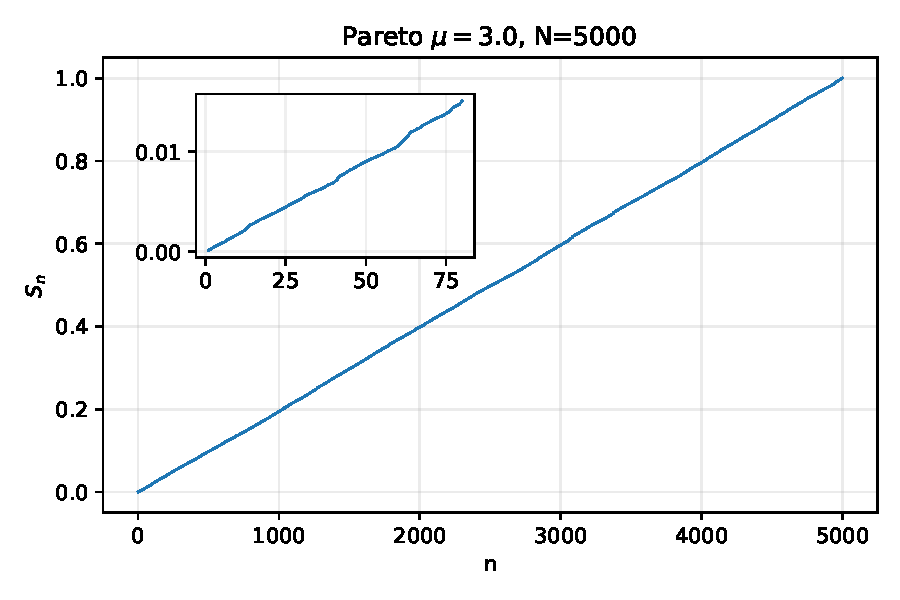
\includegraphics[width=.72\linewidth]{../figures/figure1_pareto_mu3.pdf}
\caption{Somme partielle de richesse pour $\mu=3$.}
\end{figure}

Pour $\mu=3$, la plus grande part individuelle vaut $0.247\%$ et l'inverse participation ratio vaut $Y_2=2.62\times 10^{-4}$. Le comportement est diffus: aucune richesse individuelle ne domine la population.

\begin{figure}[h]
\centering
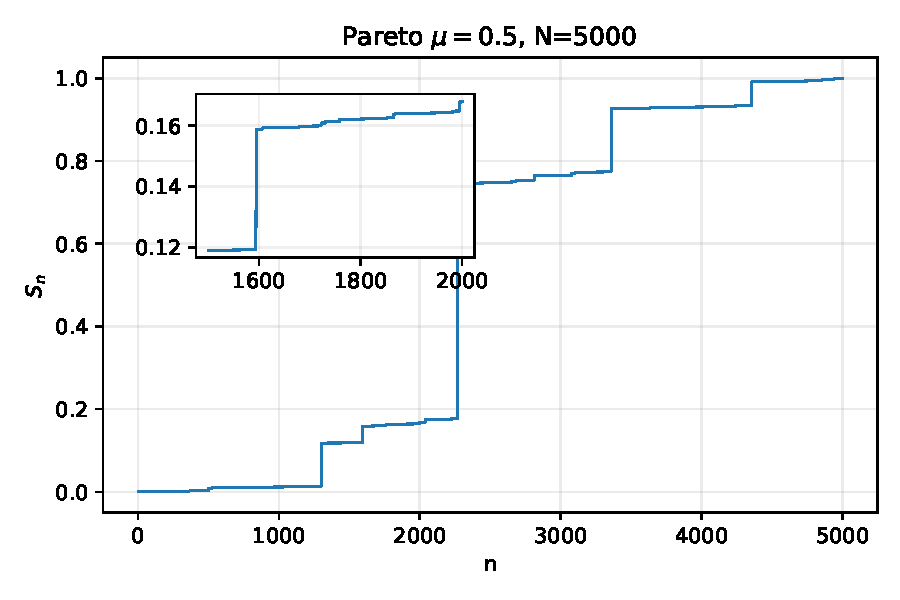
\includegraphics[width=.72\linewidth]{../figures/figure2_pareto_mu05.pdf}
\caption{Somme partielle de richesse pour $\mu=0.5$.}
\end{figure}

Pour $\mu=0.5$, la plus grande part individuelle vaut $56.9\%$ et $Y_2=0.363$. Ce résultat confirme clairement la condensation décrite par l'article: quelques agents portent une fraction macroscopique de la richesse.

\begin{figure}[h]
\centering
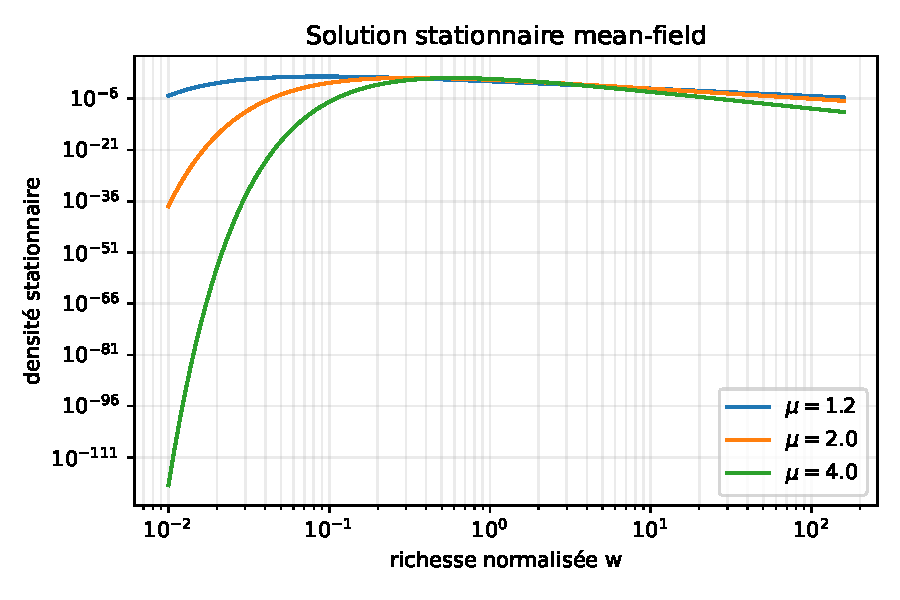
\includegraphics[width=.72\linewidth]{../figures/mean_field_stationary_density.pdf}
\caption{Densité stationnaire analytique du cas champ moyen.}
\end{figure}

La solution stationnaire de champ moyen recodée,
\[
  P(w)=\frac{(\mu-1)^\mu}{\Gamma(\mu)}\frac{\exp[-(\mu-1)/w]}{w^{1+\mu}},
\]
présente bien une queue de Pareto d'exposant $\mu=1+J/\sigma^2$.

\begin{figure}[h]
\centering
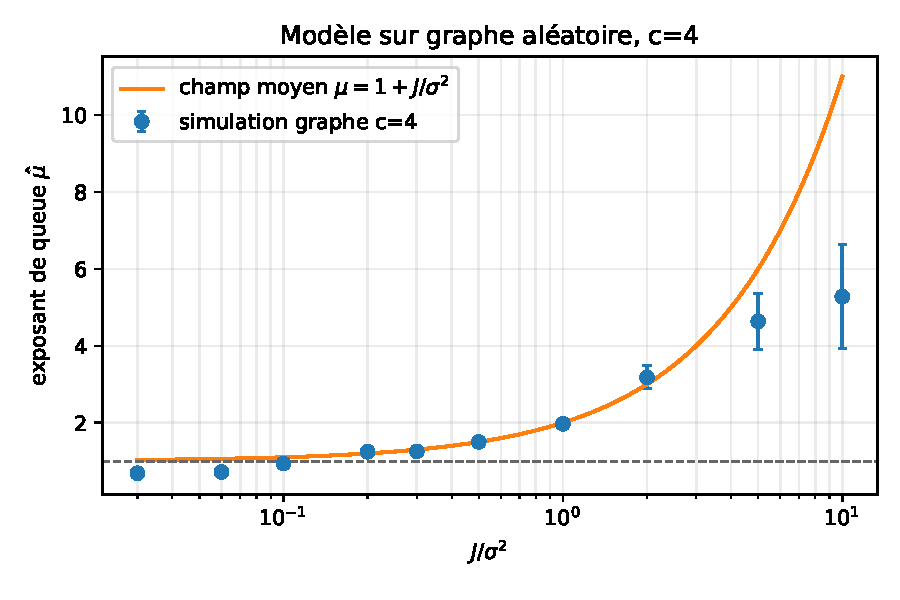
\includegraphics[width=.72\linewidth]{../figures/figure3_graph_tail_exponent.pdf}
\caption{Exposant de queue estimé sur graphe aléatoire $c=4$.}
\end{figure}

Le balayage numérique donne une transition autour de $J/\sigma^2\simeq 0.1$--$0.3$ selon l'estimation de queue. L'article annonce une transition vers $0.3$; la reproduction est donc qualitativement cohérente. Les estimations obtenues sont par exemple $\hat\mu=0.94$ pour $J/\sigma^2=0.1$, $\hat\mu=1.25$ pour $0.3$, $\hat\mu=1.97$ pour $1.0$.

\section{Analyse statistique multi-runs}

Une seconde campagne a été réalisée avec 200 tirages indépendants par couple $(N,\mu)$ pour $N\in\{1000,5000,20000\}$ et $\mu\in\{0.5,0.8,1.2,2,3\}$. Pour le modèle sur graphe, chaque point a été répété cinq fois avec $N=900$, 9000 pas et trois connectivités $c\in\{3,4,8\}$.

\begin{figure}[h]
\centering
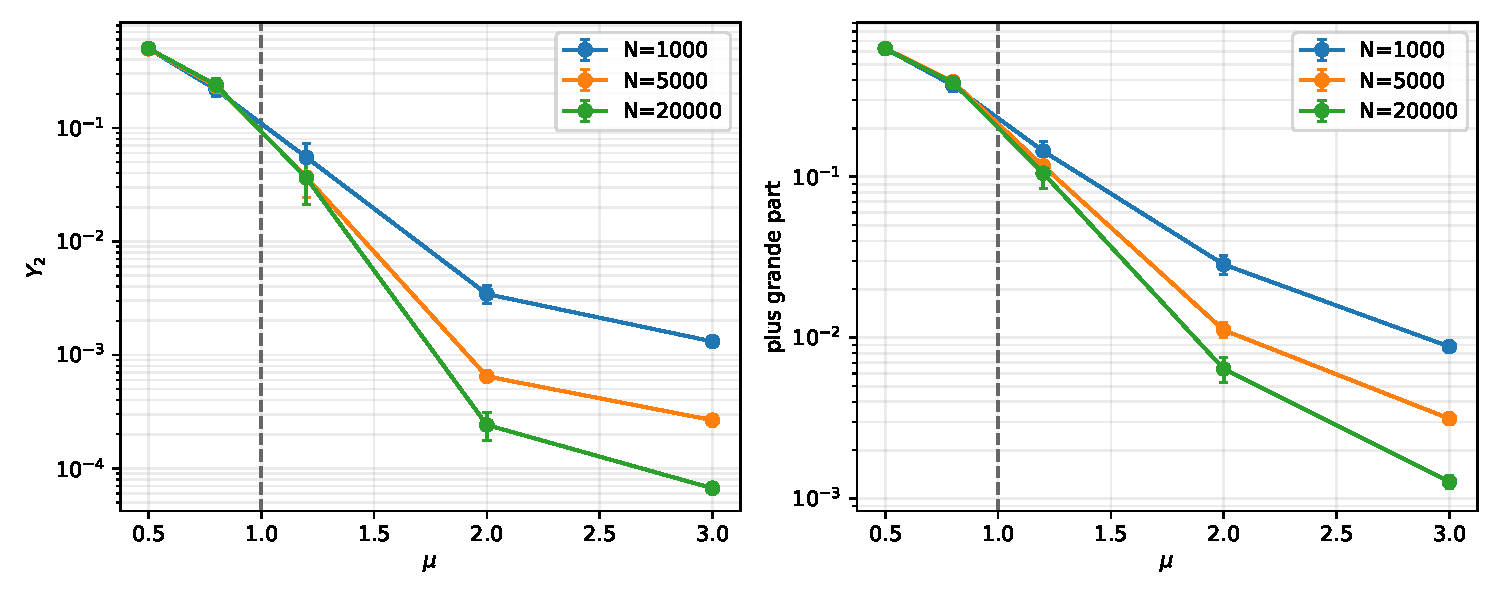
\includegraphics[width=.92\linewidth]{../figures/stat_pareto_condensation.pdf}
\caption{Moyennes et intervalles de confiance à 95\% de $Y_2$ et de la plus grande part individuelle.}
\end{figure}

\begin{table}[h]
\centering
\begin{tabular}{rrrr}
\toprule
$\mu$ & $\mathbb{E}[Y_2]$ & IC 95\% & plus grande part moyenne \\
\midrule
0.5 & 0.498 & [0.458, 0.538] & 0.628 \\
0.8 & 0.232 & [0.201, 0.263] & 0.389 \\
1.2 & 0.0369 & [0.0242, 0.0496] & 0.117 \\
2.0 & $6.47\,10^{-4}$ & [$5.92\,10^{-4}$, $7.02\,10^{-4}$] & 0.0112 \\
3.0 & $2.66\,10^{-4}$ & [$2.62\,10^{-4}$, $2.70\,10^{-4}$] & 0.00314 \\
\bottomrule
\end{tabular}
\caption{Résultats pour $N=5000$, 200 répétitions.}
\end{table}

Pour $\mu=0.5$, la valeur théorique $\mathbb{E}[Y_2]=1-\mu=0.5$ est retrouvée presque exactement. Pour $\mu<1$, $Y_2$ et la plus grande part restent d'ordre un quand $N$ augmente. Pour $\mu>1$, ils décroissent avec $N$. La transition de condensation est donc confirmée statistiquement, et pas seulement sur un tirage représentatif.

\begin{figure}[h]
\centering
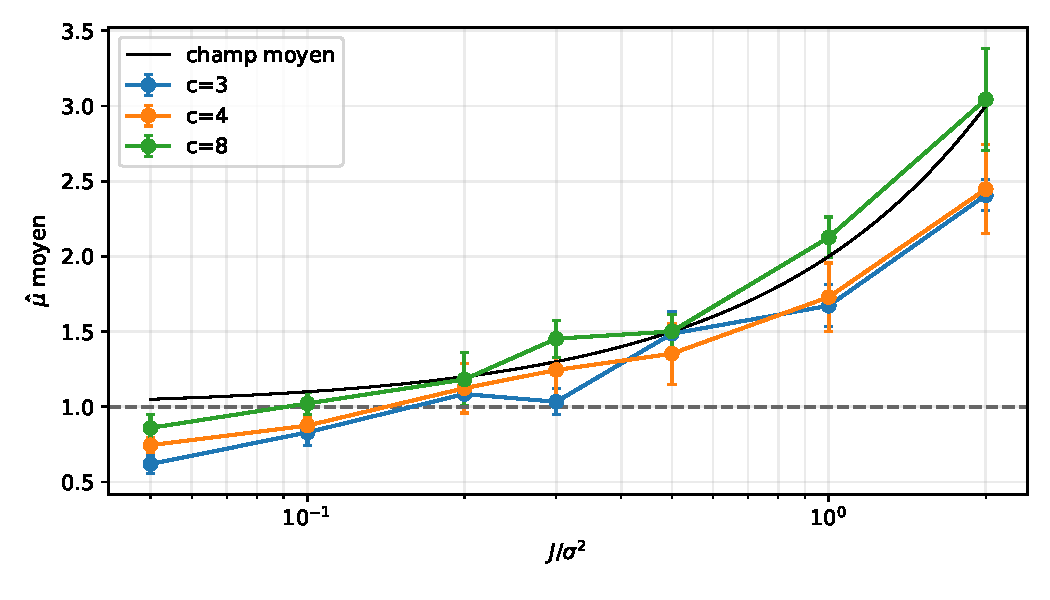
\includegraphics[width=.82\linewidth]{../figures/stat_graph_connectivity.pdf}
\caption{Exposant de queue moyen et IC 95\% selon $J/\sigma^2$ et la connectivité.}
\end{figure}

Pour $c=4$, les moyennes sont $\hat\mu=0.745$ à $J/\sigma^2=0.05$, $0.875$ à $0.1$, $1.124$ à $0.2$ et $1.245$ à $0.3$. Le franchissement de $\mu=1$ se situe donc statistiquement entre $0.1$ et $0.3$, compatible avec le seuil d'environ $0.3$ annoncé. L'augmentation de la connectivité rapproche globalement le résultat de la prédiction de champ moyen, mais les intervalles restent larges dans le régime condensé.

\section{Points insuffisamment décrits et choix faits}

\begin{itemize}
  \item L'article ne donne pas $N$, le pas de temps, la durée de relaxation, ni la méthode précise d'estimation de $\mu$ pour la figure 3. J'ai choisi $N=900$, $dt=0.01$, 9000 pas dont 3000 de transitoire, et un estimateur de Hill sur les 8\% supérieurs.
  \item Le graphe aléatoire est décrit par sa connectivité moyenne $c=4$; j'ai utilisé un graphe d'Erdős--Rényi symétrique, puis reconnecté les rares noeuds isolés.
  \item Les chocs multiplicatifs gaussiens sont intégrés par une étape exponentielle suivie de l'échange linéaire; ce choix conserve la positivité des richesses, ce qui est essentiel pour mesurer une queue de Pareto.
\end{itemize}

\section{Conclusion}

Les résultats centraux sont confirmés avec support statistique. Les 200 répétitions par point retrouvent notamment $\mathbb{E}[Y_2]=1-\mu$ dans le régime condensé et la disparition de $Y_2$ avec $N$ pour $\mu>1$. La simulation sur graphe aléatoire retrouve une transition du bon ordre de grandeur et montre que la connectivité réduit l'écart au champ moyen. La comparaison quantitative fine de la figure 3 reste limitée par les détails numériques absents de l'article et par l'incertitude élevée des estimateurs de queue.

\end{document}
